% Gemini theme
% https://github.com/anishathalye/gemini
%
% We try to keep this Overleaf template in sync with the canonical source on
% GitHub, but it's recommended that you obtain the template directly from
% GitHub to ensure that you are using the latest version.

\documentclass[final, 20pt]{beamer}

% ====================
% Packages
% ====================

\usepackage[T1]{fontenc}
\usepackage{lmodern}
% \usepackage[size=custom,width=120,height=72,scale=1.0]{beamerposter}
\usepackage[size=a1,scale=1.3]{beamerposter}
\usetheme{gemini}
\usecolortheme{gemini}
\usepackage{graphicx}
\graphicspath{ {./images/} }
\usepackage{booktabs}
\usepackage{tikz}
\usepackage{pgfplots}
%\usepackage{subfigure}
\usepackage{caption}
\usepackage{subcaption}

\usepackage[export]{adjustbox}
\usepackage{wrapfig}
\usepackage{lipsum}
% ====================
% Lengths
% ====================

% If you have N columns, choose \sepwidth and \colwidth such that
% (N+1)*\sepwidth + N*\colwidth = \paperwidth
\newlength{\sepwidth}
\newlength{\colwidth}
\setlength{\sepwidth}{0.025\paperwidth}
\setlength{\colwidth}{0.3\paperwidth}

\newcommand{\separatorcolumn}{\begin{column}{\sepwidth}\end{column}}

% ====================
% Title
% ====================

\title{Construction/Operation of Two Hexacopters for Autonomous Landing}

\author{Joshua Springer}

\institute[shortinst]{Reykjavík University}

% ====================
% Body
% ====================

\begin{document}

\begin{frame}[t]
\begin{columns}[t]
\separatorcolumn

\begin{column}{\colwidth}

  \begin{block}{Overview}
    This project tests an autonomous landing algorithm based on computer vision and fiducial markers.\cite{AL_thesis}
    Two Tarot 680 Hexacopters enable real world testing of autonomous navigation techniques developed in simulation.
    A landing pad is marked with fiducial markers which are recognized by the drone's onboard camera.
    The gimbal automatically aims the camera at the landing pad to track it during descent.
    The landing software then directs the drone to descend towards the landing pad.
  \end{block}

  \begin{alertblock}{Components}

    \heading{Standard Drone Components}
    All drone electronics (e.g. motors, speed controllers, propellers, power electronics, RC Receiver, telemetry radio) are mounted on the Tarot 680 Pro hexacopter body.

    \heading{Computational Components}
    \begin{itemize}
      \item \textbf{Raspberry Pi 3 B+:} runs the ArduPilot flight software and ROS.
      \item \textbf{Navio2 Hat:} provides IMU data and control signal interfaces.
      \item \textbf{Companion board:} image processing, fiducial marker systems, coordinate system transforms. One drone uses a Google Coral Dev board and the other uses an NVIDIA Jetson Nano.
    \end{itemize}

    \begin{figure}
      \includegraphics[width=0.45\linewidth]{jetson_electronics}
      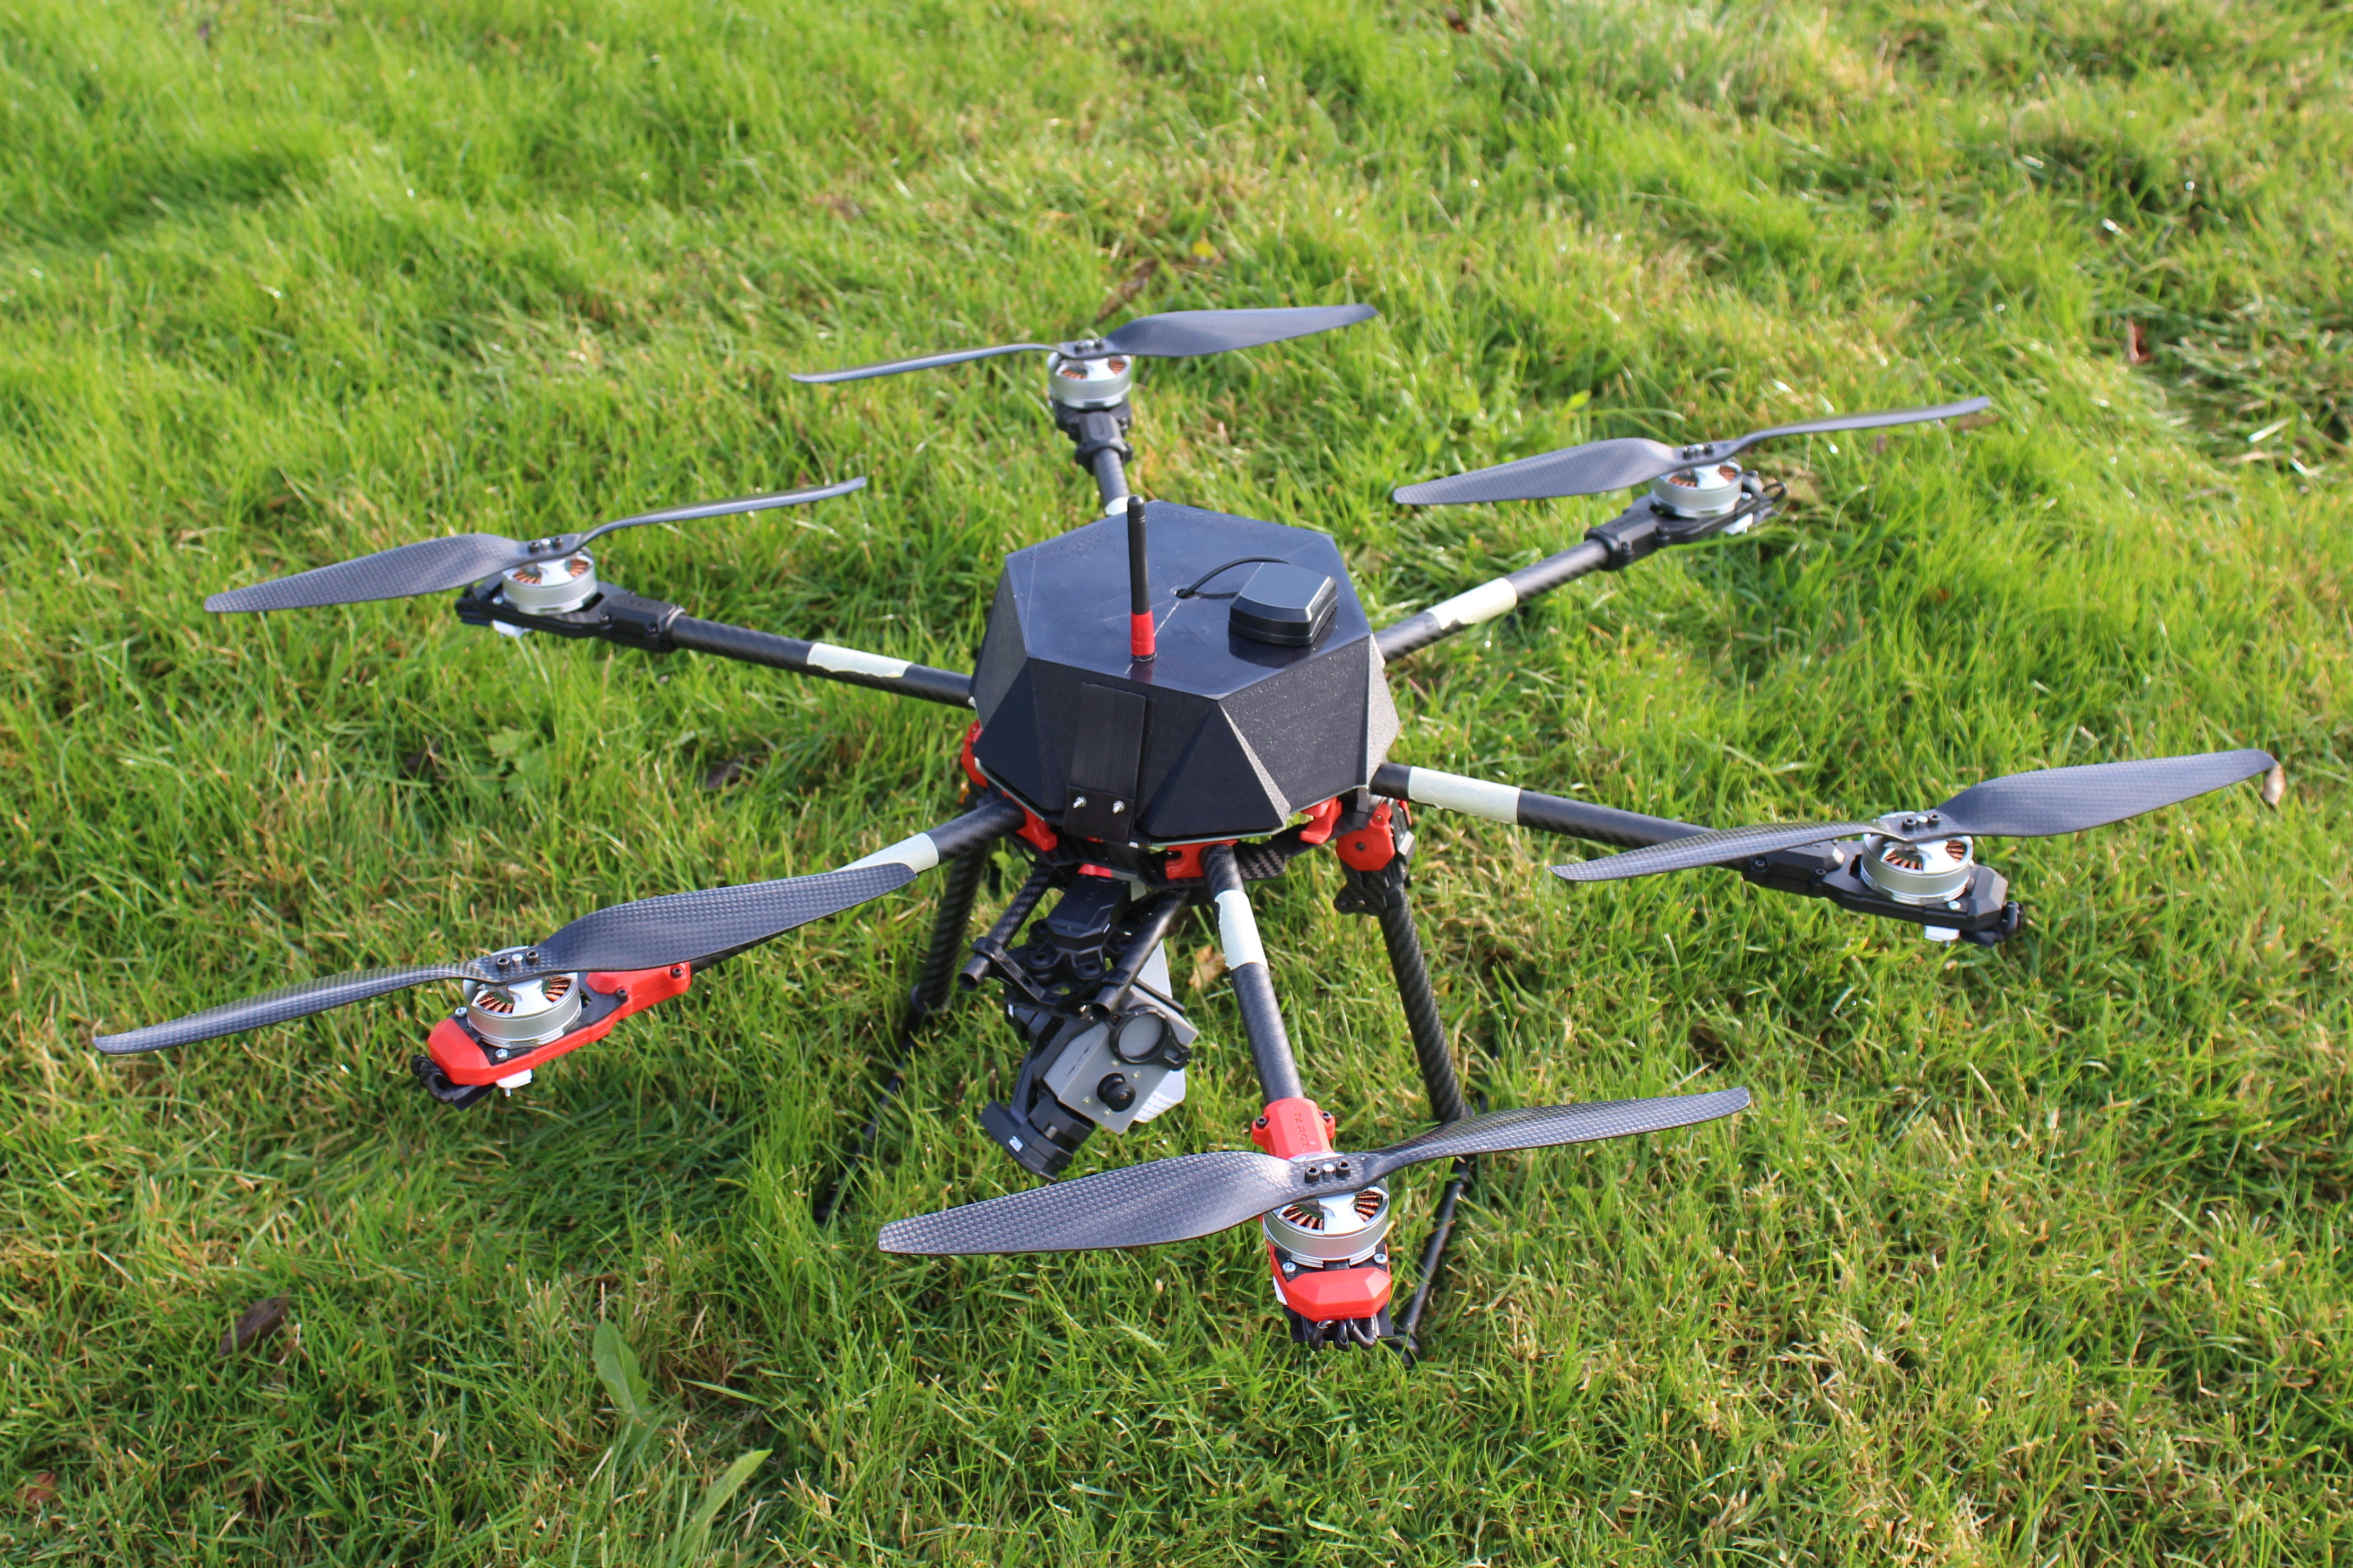
\includegraphics[width=0.45\linewidth]{jetson_drone.jpg}
    \end{figure}

    \heading{Custom 3D-Printed Components}

    \begin{figure}
      \centering
      \begin{subfigure}[b]{0.33\textwidth}
        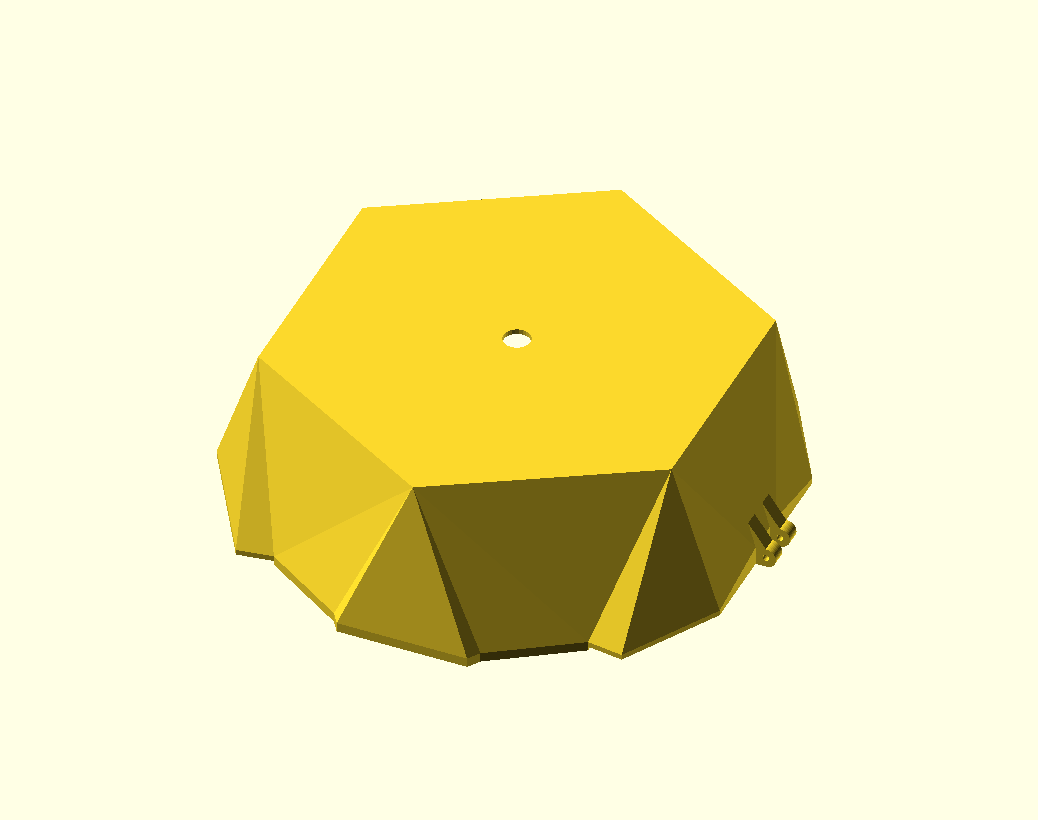
\includegraphics[width=\textwidth]{canopy.png}
        \caption*{Protective Canopy.}
      \end{subfigure}
      \hspace{1cm}
      \begin{subfigure}[b]{0.33\textwidth}
        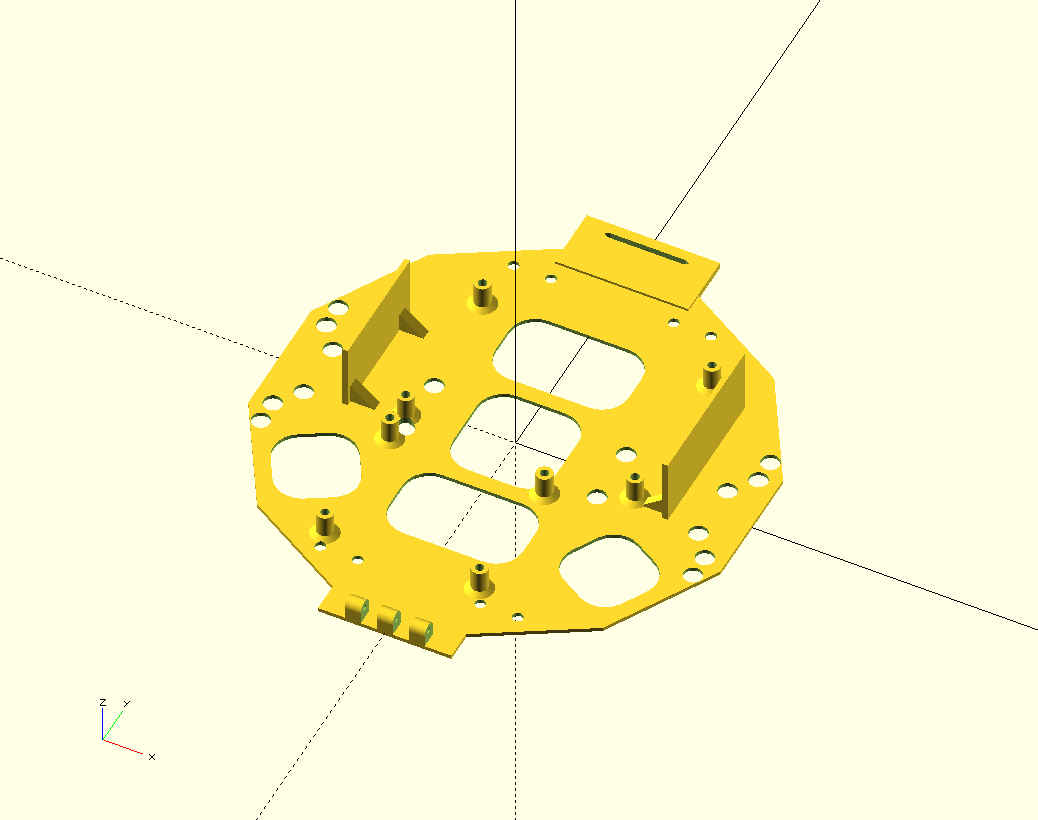
\includegraphics[width=\textwidth]{component_mounting_plate.png}
        \caption*{Component mounting plate.}
      \end{subfigure}

      \begin{subfigure}[b]{0.33\textwidth}
        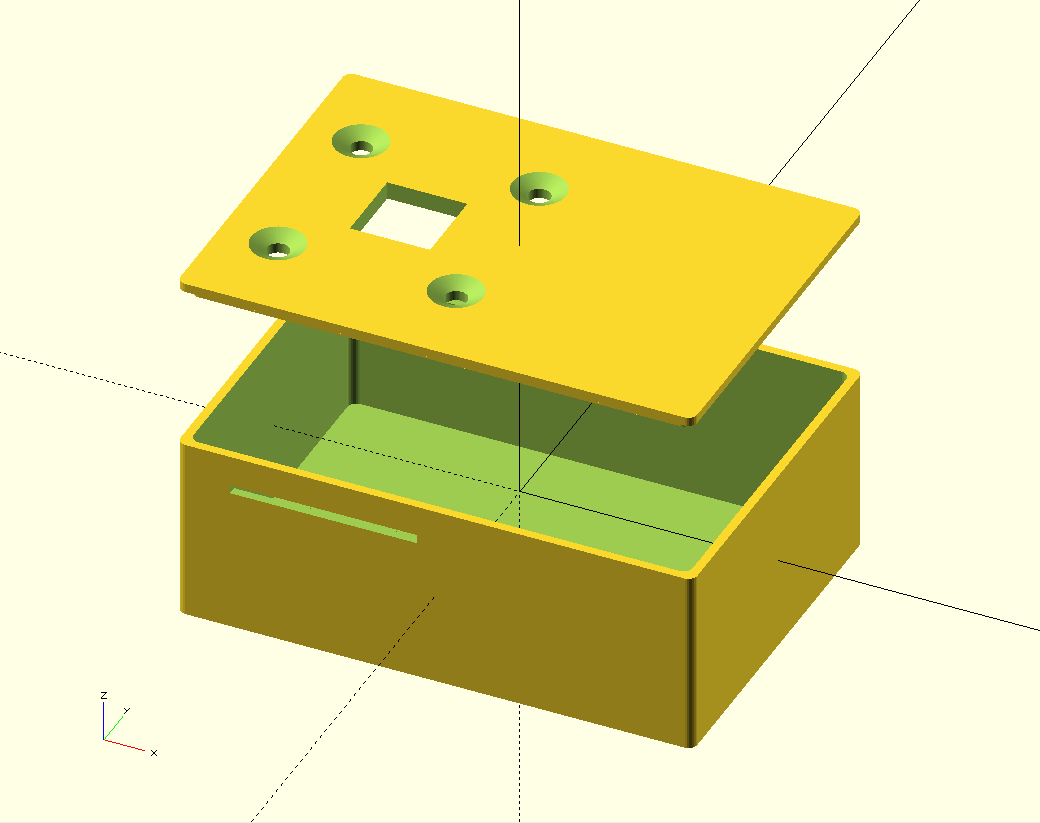
\includegraphics[width=\textwidth]{coral_case.png}
        \caption*{Google Coral camera case.}
      \end{subfigure}
      \hspace{1cm}
      \begin{subfigure}[b]{0.33\textwidth}
        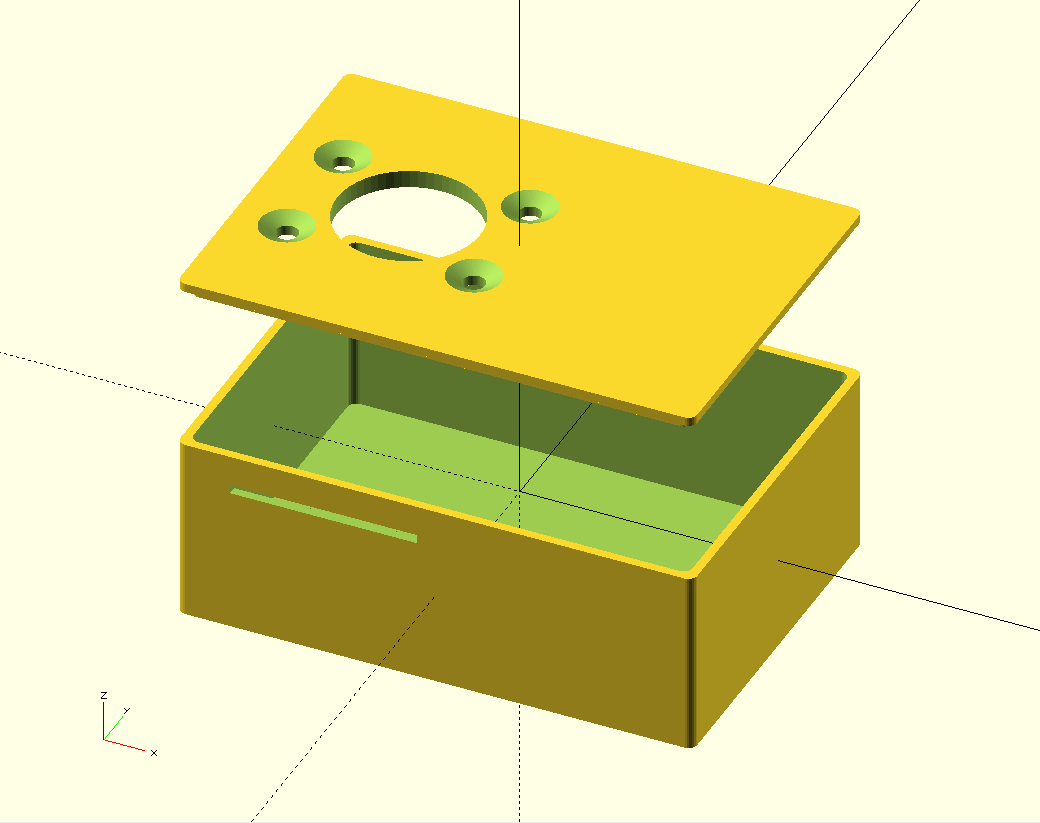
\includegraphics[width=\textwidth]{nano_case.png}
        \caption*{Jetson Nano camera case.}
      \end{subfigure}
    \end{figure}
  \end{alertblock}

\end{column}

\separatorcolumn

\begin{column}{\colwidth}

  \begin{block}{Power and Data Flow}
        The drones have two power systems to isolate the computational electronics from voltage spikes/drops caused by the motors and gimbal.
        \begin{figure}
          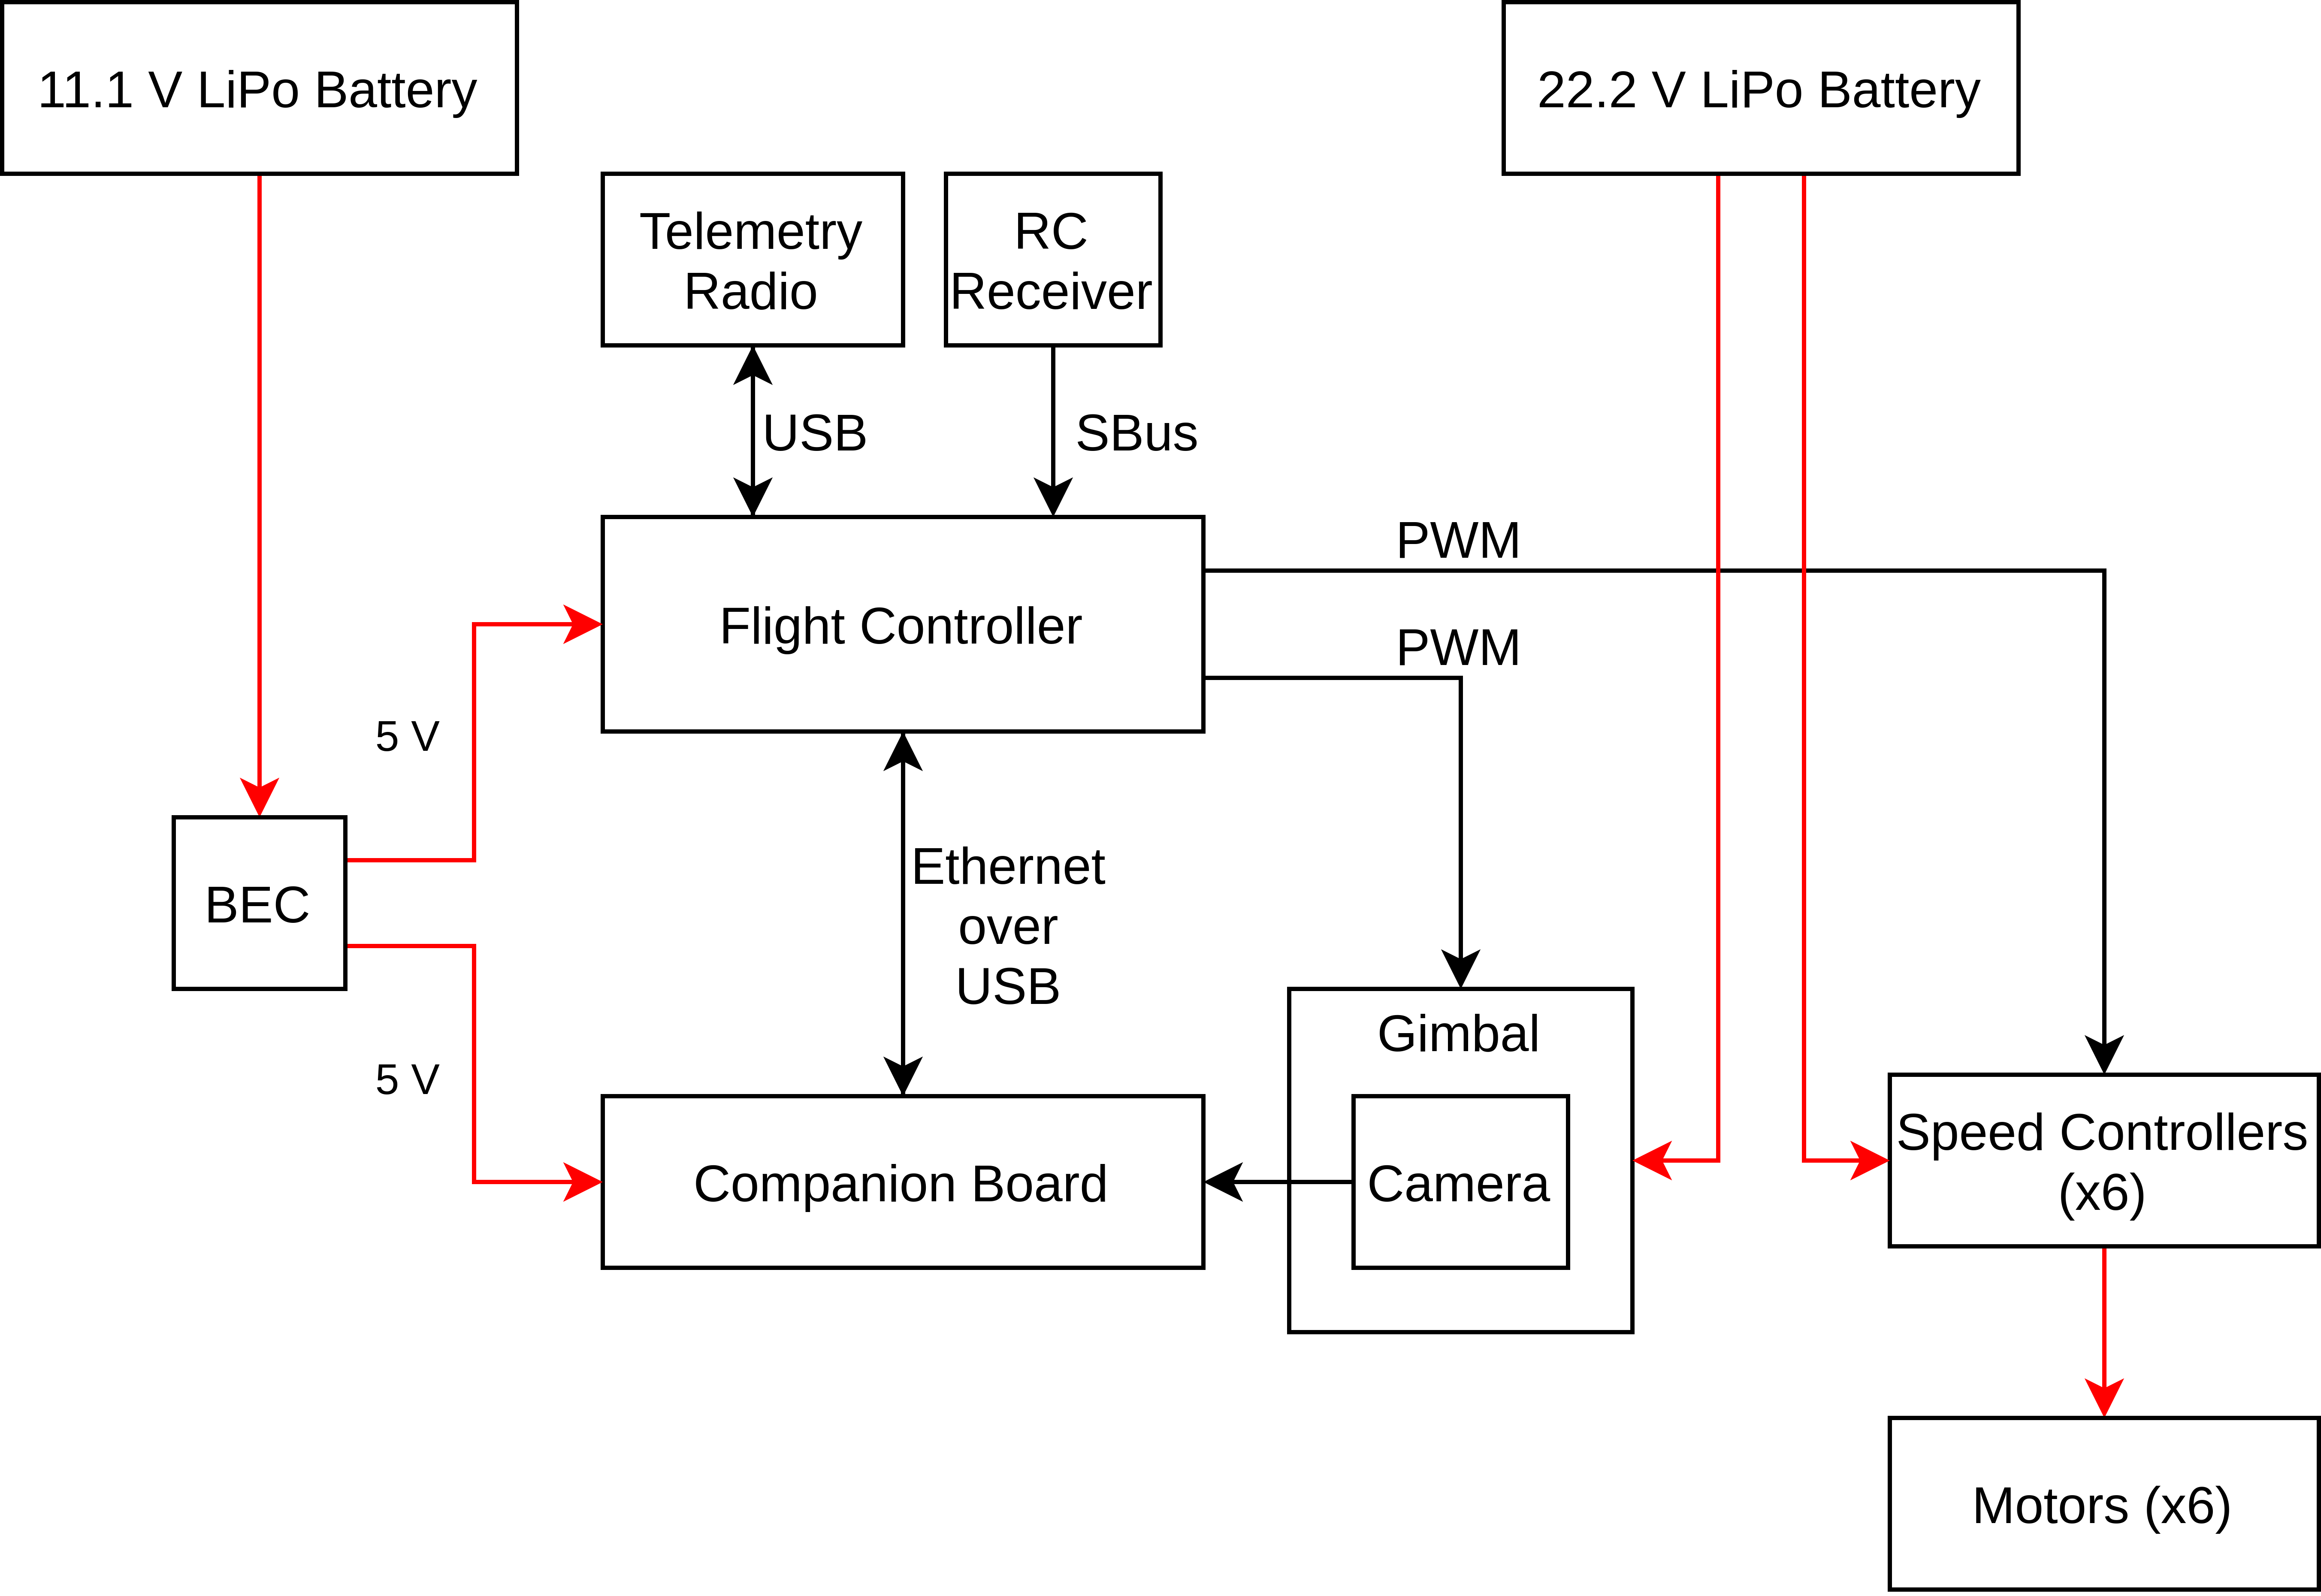
\includegraphics[width=0.6\textwidth]{hardware.png}
%          \caption{Power flow and control signals.}
        \end{figure}

        \vspace{-1.5cm}
        \heading{Data Flow}
        \begin{itemize}
          \item \textbf{Camera module:} provides a high-quality video image.
          \item \textbf{\texttt{gscam}:} pre-processes the image (lowering resolution, flipping).
          \item \textbf{\texttt{landing\_controller}:} generates a target position for the drone.
          \item \textbf{\texttt{gimbal\_controller}:} tracks the landing pad by aiming the camera.
          \item \textbf{MAVROS:} translates ROS messages to ArduPilot messages.
          \item \textbf{ArduPilot:} controls the drone based on MAVROS commands.
        \end{itemize}

        \begin{figure}
            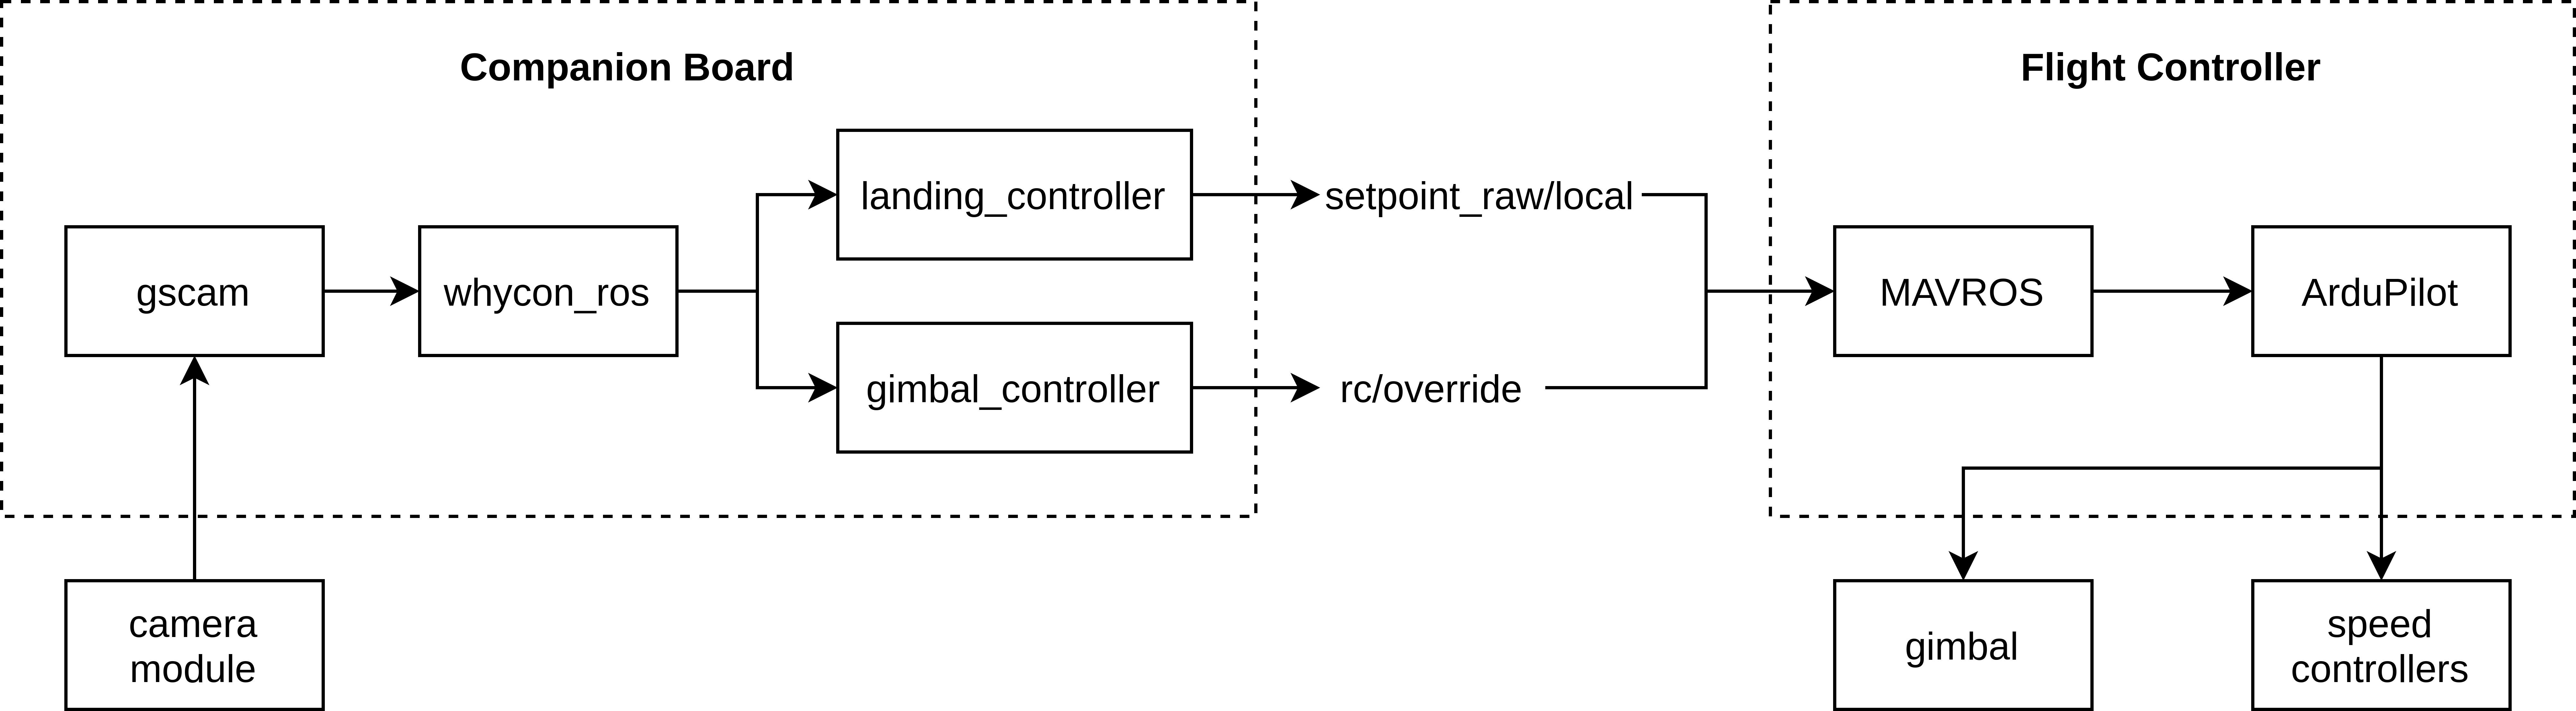
\includegraphics[width=0.9\textwidth]{data_flow.png}
        \end{figure}
  \end{block}

  \begin{block}{Landing Pad}

    \vspace{0.5cm}
    \begin{columns}
      \begin{column}{0.65\textwidth}
        Fiducial markers (top: April Tag\cite{apriltag_paper}, bottom: WhyCon\cite{whycon_paper}) allow the drone to determine its position relative to the landing pad using only a normal RGB camera.

        \begin{itemize}
          \item \textbf{April Tag:} provides accurate pose estimation at close range, when the WhyCon marker is too big for the camera to fully see. Eventually it was abandoned for consuming excessive CPU time.
          \item \textbf{WhyCon:} provide easier/faster recognition at long range. The center of the WhyCon marker is the target landing site.
        \end{itemize}
      \end{column}
      \begin{column}{0.3\textwidth}
        \fbox{
\includegraphics[angle=180, width=7cm]{landing_pad.png}}
      \end{column}
    \end{columns}

    The landing pad graphic is printed on white paper and attached to a rigid piece of plastic.

  \end{block}

\end{column}

\separatorcolumn

\begin{column}{\colwidth}

  \begin{alertblock}{Performance}

    \heading{Flight}
      Both drones are very stable and reliable, with pitch/roll variance of $\approx 3^{\circ}$ in high wind, as shown below.
      They have safe flight times of about 15 minutes and enough thrust to carry additional instruments/sensors.
      \begin{figure}
        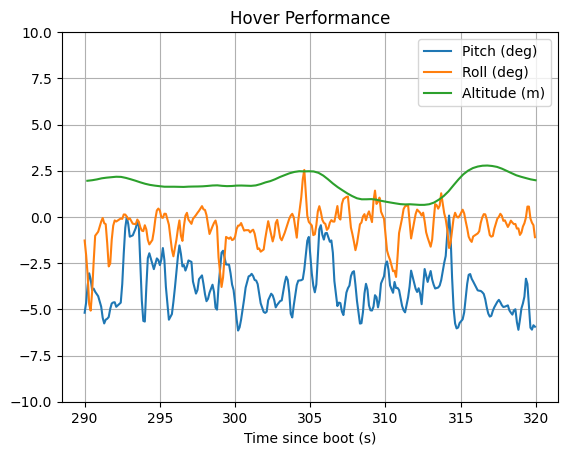
\includegraphics[width=0.3575\textwidth]{stability.png}
        \hspace{1cm}
        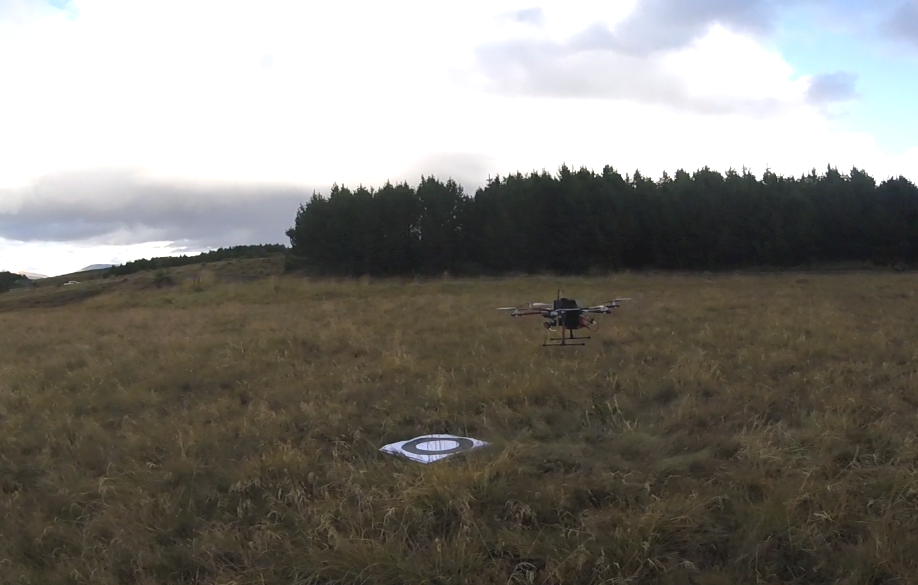
\includegraphics[width=0.45\textwidth]{drone_in_flight.png}
        \caption*{Left: pitch, roll, altitude during hover. Right: flight (Scan QR in top right for video!)}
      \end{figure}

    \vspace{-0.5cm}
    \heading{Autonomous Landing}

      \begin{itemize}
        \item Both drones are able to track the landing pad during lab testing.
        \item Jetson Nano has power issues in field testing and is unable to track.
        \item Google Coral drone is able to track and approach the landing pad.
        \item WhyCon system has issues with orientation at close range (beyond the scope of this project).
      \end{itemize}

%      Autonomous landing has nearly been achieved, but some adjustments to the fiducial marker system must be made to improve pose estimation reliability.

  \end{alertblock}

  \begin{block}{Future Work}

    \begin{itemize}
      \item \textbf{Change pose estimation system:} either fix WhyCon orientation issues, or develop a more robust solution (new marker, deep learning model).
      \item \textbf{More autonomous missions:} landing, navigation, data collection, mapping, object recognition/tracking.
      \item \textbf{Add more instruments/sensors:} depth/hyperspectral cameras.
    \end{itemize}

  \end{block}

  \begin{alertblock}{Contact Us}
    We want to hear from you!
    If you are interested in participating or have a project idea involving drones, feel free to contact us:

    \begin{center}
%    \begin{tabular}{|l|l|}
    \begin{tabular}{|ll|}
        \hline
        Joshua Springer & joshua19@ru.is\\%\hline
        Marcel Kyas & marcel@ru.is\\\hline
    \end{tabular}
    \end{center}
  \end{alertblock}

  \begin{block}{References}
    \vspace{-0.5cm}
%    \nocite{*}
    \bibliographystyle{ieeetr}
    \footnotesize{\bibliography{poster}}

  \end{block}

\end{column}

\separatorcolumn
\end{columns}
\end{frame}

\end{document}
